\chapter{Architecture and implementation}\label{chapter:architecture}

Building on the designed abstraction and algorithms from previous chapters, a prototype application is developed to serve as a proof of concept and to demonstrate the feasibility. The application presents a simple graphical user interface in the form of a single-page website. The background application provides an interface for communication, all translation logic along with integration tests. Internally, the application adheres to design patterns proposed in earlier chapters. It implements parsers constructing the intermediate representation, which builders subsequently translate to user-selected \acrshort{orm}.

The prototype application currently supports three \acrshort{orm} frameworks -- Dapper, NHibernate, and \acrshort{efcore}. Those were chosen for their criteria analyzed in Chapter~\ref{chapter:ormcomparison}, mainly their popularity and variety in mapping and querying. Dapper represents macro \acrshort{orm}(s), with its lack of mapping and support for only \acrshort{sql} queries. \acrshort{efcore} was chosen for its feature set, extensive \acrshort{linq} coverage, and attribute mapping. NHibernate completes this set with a unique mapping format in \acrshort{xml} files.

Figure~\ref{fig:supported_directions} visualizes currently supported translation directions. Entity and mapping configurations are translatable between all the three \acrshort{orm}(s). The tool can translate \acrshort{efcore}'s \acrshort{linq} queries into Dapper's \acrshort{sql}.

\begin{figure}[!htp]
  \centering
  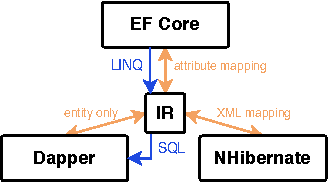
\includegraphics[scale=1.5]{thesis/img/thesis/06_supported_directions.drawio.pdf}
  \caption{Supported translation directions}
  \label{fig:supported_directions}
\end{figure}

\section{Application architecture}
The application is written in .NET 8 and is structured into multiple projects. In .NET, each project represents a distinct unit of compilation, functioning as an application module with explicitly defined dependencies. These projects are grouped within a .NET solution file, which can be managed and run through Visual Studio\footnote{\url{https://visualstudio.microsoft.com/}} or any other \acrshort{ide}.\footnote{\url{https://learn.microsoft.com/en-us/visualstudio/ide/solutions-and-projects-in-visual-studio}} 

Figure~\ref{fig:app_architecture} illustrates the application's decomposition into projects and project folders. Arrows in the figure demonstrate dependencies between projects.

There are three distinct project types used. The first is an ASP.NET\footnote{\url{https://dotnet.microsoft.com/en-us/apps/aspnet}} web project used in the \texttt{ORMConvertorAPI} to provide data and translation interfaces to the frontend. Although the frontend is technically independent and runs within a browser, its static source files are served by this project. The second project type is a testing project based on the xUnit framework,\footnote{\url{https://xunit.net/}} used by the \texttt{Tests} project to perform integration tests. Integration tests are implemented for each translation direction as well as their combination. The remaining projects belong to the third category, C\# class library projects, which are not executable and can only be utilized through references within executable projects. 

\begin{figure}[!htp]
  \centering
  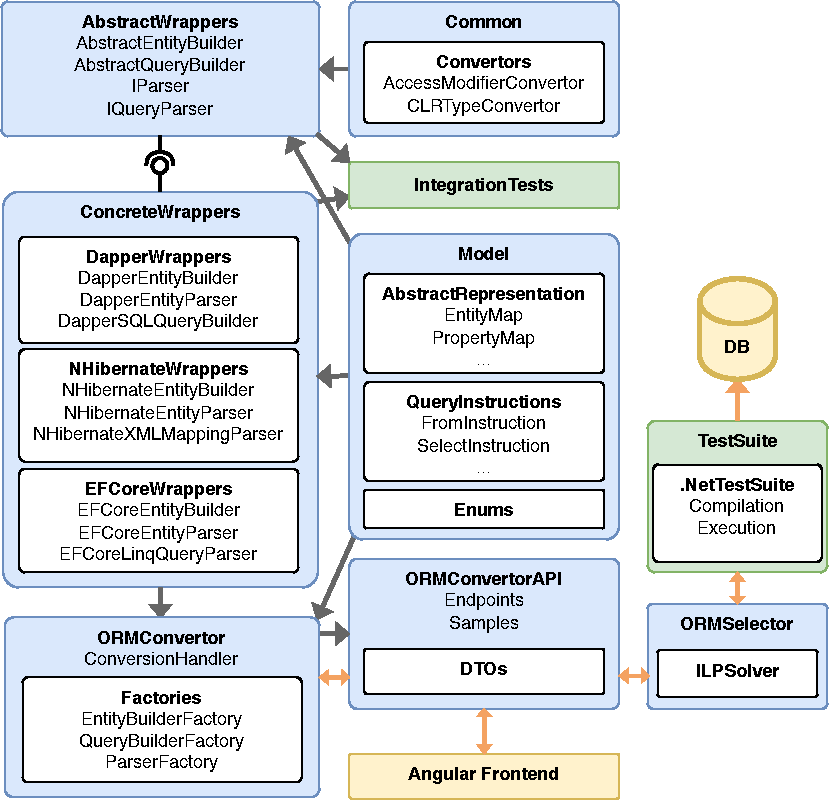
\includegraphics[scale=1]{thesis/img/thesis/06_architecture.drawio.pdf}
  \caption{Application architecture}
  \label{fig:app_architecture}
\end{figure}

\texttt{Model} is a first representative of library project. It represents a central project containing domain models. It houses models for entity mapping intermediate representation designed in Chapter~\ref{chapter:entity_translation} along with immutable records representing instructions for queries from Chapter~\ref{chapter:query_translation}. In addition, it includes enumerations, exception types, and other objects the application depends on. The project is referenced by almost all others as it is essential to application function.

\texttt{AbstractWrappers} is another library project. As such, it defines interfaces for builders and parsers. As builders share some common functionality, they are declared as \textit{abstract} classes with certain methods implemented. Parsers only declare an interface without any implementation. Concrete wrappers are then implemented in \texttt{ConcreteWrappers} project folder. Each ORM has its own project to isolate them and to decouple dependencies.

Finally, the main translation algorithm is defined in \texttt{ORMConvertor} (library) project in the \texttt{ConversionHandler} class. The class is responsible for receiving source \acrshort{orm} inputs, orchestrating appropriate parsers and builders, and returning correct output. \texttt{ConversionHandler} does not work with specific implementations, it only accesses them through interfaces. Factories are responsible for returning the correct wrappers and instantiating them. This class is a direct implementation of Algorithm~\ref{alg:translation_alg}.

\section{Wrappers}
Each wrapper, either a parser or builder, effectively serves as an adapter, translating between the specific interface of an \acrshort{orm} and the intermediate representation. Their function aligns with the \textit{adapter} pattern, enabling interoperability between otherwise incompatible representations.

Entity parsers for each framework follow a similar approach, leveraging the Roslyn syntax analyzer to extract class information. The Dapper parser handles only entity structure, while the \acrshort{efcore} parser also interprets attribute-based mapping. NHibernate employs two separate parsers: one mirrors the behaviour of the Dapper parser by processing only the entity, while the other parses the \acrshort{xml} mapping using \acrshort{linq} to \acrshort{xml}.\footnote{\url{https://learn.microsoft.com/en-us/dotnet/standard/linq/linq-xml-overview}}

Currently, only parsing of \acrshort{efcore} \acrshort{linq} queries is supported. Due to the flexibility of \acrshort{linq}, in method order and lambda expressions, parsing is fairly complex. The implementation extends \texttt{CSharpSyntaxTree}, overriding the \texttt{Visit} method to analyze method call expressions. 

Entity builders follow an identical strategy, populating string templates and collecting the final structure in \texttt{StringBuilder}. The NHibernate builder separately constructs the entity class and its corresponding \acrshort{xml} mapping, producing two outputs.

As for query builder, only the Dapper \acrshort{sql} builder is implemented. It uses \texttt{StringBuilder} to sequentially assemble query components, while a dedicated visitor class handles concrete syntax generation.


\section{Interaction}
To allow easy user interaction, the translation tool has a minimal frontend. It also exposes a \acrshort{rest} \acrshort{api} allowing for programmatic access or automation. Documentation for the \acrshort{api} is auto-generated using Swagger\footnote{\url{https://swagger.io/}} and is available at \texttt{/orm/swagger} endpoint.

Figure~\ref{fig:tool_interface} showcases the appearance of the web page when opened. It is split into two panes. On the left, the user selects the source \acrshort{orm} and inputs the required data. Inputs change based on the selected framework and implemented wrappers. In the figure, NHibernate appears by default, requiring C\# entity and \acrshort{xml} mapping. For easier testing, sample inputs can be loaded for each framework, using the \texttt{'Fill~Samples'} button. Figure~\ref{fig:tool_interface_translated} demonstrates translation from \acrshort{efcore} to Dapper. Entity gets translated, losing all mapping in the process as Dapper does not support it. The \acrshort{linq} query is converted into \acrshort{sql}.

\begin{figure}[!htp]
  \centering
  \fbox{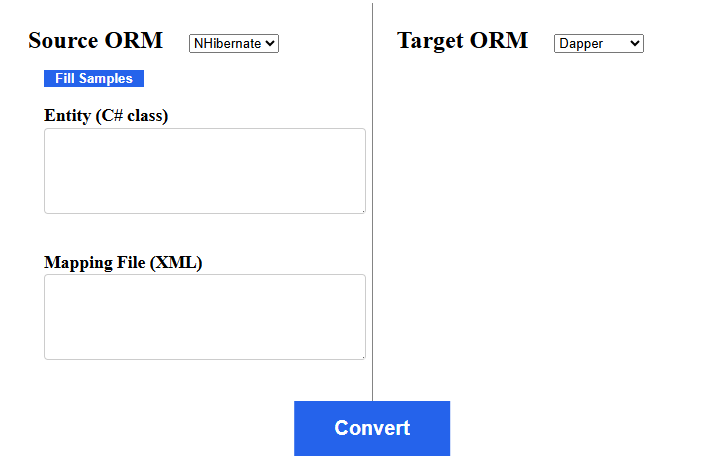
\includegraphics[scale=1]{thesis/img/thesis/06_app_ui.png}}
  \caption{Interface of the translation tool}
  \label{fig:tool_interface}
\end{figure}

\afterpage{
\begin{landscape}
\begin{figure}[!htp]
  \centering
  \fbox{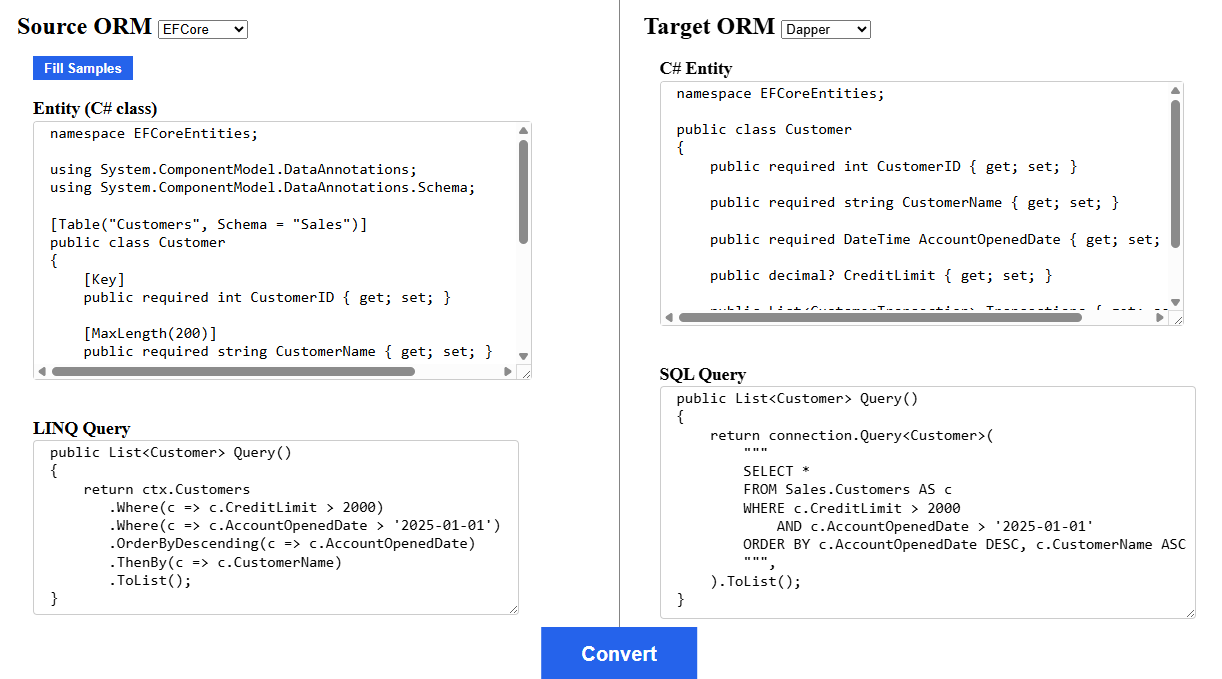
\includegraphics[width=0.9\textwidth]{thesis/img/thesis/06_app_ui_translated.png}}
  \caption{Translation tool interface when translating from \acrshort{efcore} to Dapper}
  \label{fig:tool_interface_translated}
\end{figure}
\end{landscape}
}

\section{Deployment}
The application can be run in two main ways. The more user-friendly approach is to open the solution file \texttt{ORMConvertor.sln} in Visual Studio. \texttt{ORMConvertorAPI} has to be set as the startup project, if not selected by default. The app can be launched in \texttt{Debug} configuration for development or compiled in \texttt{Release} configuration for production. Only the \texttt{http} launch profile\footnote{defined in \texttt{ORMConvertorAPI/Properties/launchSettings.json} file} has been configured and tested. The application can be started with \texttt{CTRL + F5} to run without debugging or \texttt{F5} to launch with the debugger. A browser window should open automatically.

Alternatively, the application can be started using .NET \acrshort{cli} using the command in Listing~\ref{lst:run_app}. All options must be provided (i.e., are required). This approach does not open a browser automatically. Instead, the local \acrshort{url} is printed to the console (typically \texttt{http://localhost:5072/orm/}).
\begin{lstlisting}[numbers=none,caption=Application launch command,label=lst:run_app]
dotnet run --configuration Release --launch-profile http --project ORMConvertorAPI/ORMConvertorAPI.csproj
\end{lstlisting}

Tests can be executed via the Visual Studio's \texttt{Test Explorer} window or with a .NET \acrshort{cli} command in Listing~\ref{lst:run_tests}. The output displays the results of succeeded and failed tests. Tests are also run automatically on each commit using a GitHub Actions\footnote{\url{https://github.com/features/actions}} pipeline. The pipeline configuration is located in the \texttt{.github} folder at the root of the repository.
\begin{lstlisting}[numbers=none,caption=Test execution command,label=lst:run_tests]
dotnet test Tests/Tests.csproj --configuration Release
\end{lstlisting}

The Angular frontend is precompiled and served by the ASP.NET web server running the API. To prepare the frontend, its source files must be compiled and copied to the \texttt{wwwroot} directory, from which they are served as static files. This process is performed by executing the commands in Listing~\ref{lst:angular_windows} for Windows or Listing~\ref{lst:angular_linux} for Linux in the \texttt{ORMConvertorAPI/frontend} directory.

\begin{lstlisting}[numbers=none,caption=Angular compilation commands (Windows),label=lst:angular_windows]
npm install
ng build --configuration "production" --base-href "/orm/" --deploy-url "/orm/" && rmdir /s /q "..\wwwroot" && mkdir "..\wwwroot" && xcopy /s /e /y "dist\browser\*" "..\wwwroot\"
\end{lstlisting}

\begin{lstlisting}[numbers=none,caption=Angular compilation commands (Linux),label=lst:angular_linux]
npm install
ng build --configuration "production" --base-href "/orm/" --deploy-url "/orm/" && rm -rf "../wwwroot" && mkdir "../wwwroot" && cp -r dist/browser/* ../wwwroot/
\end{lstlisting}

\section{Future expansions}
The implemented prototype demonstrates the feasibility and practicality of the designed abstractions and translation mechanism. While the prototype serves as a proof of concept, it remains far from a complete implementation. To enhance the tool's capabilities and address its current limitations, several directions for future development can be identified. 

The tool currently supports three \acrshort{orm}(s) in a limited manner. Existing wrappers cover only a subset of each framework's features. Continued development could improve usability and extend the tool's applicability in real-world scenarios. Support does not need to remain limited to just the three selected frameworks or even the .NET ecosystem. 

The current implementation also lacks support for connecting to an underlying database and performing metadata queries, as proposed in Chapter~\ref{chapter:entity_translation}. In addition, the tool could potentially scaffold database schema directly, converting them into the intermediate representation without any initial input, speeding up new application development, migration of applications without \acrshort{orm}(s), or even enabling migration from a different language.

Furthermore, the current implementation does not include the condition trees in abstract query instructions proposed in Section~\ref{sec:asbtract_instructions}. This limits the tool's capability to translate complex query filters.
 
The user interface is another clear area for improvement. It could support automatic input framework detection to simplify the workflow. Integration with the Advisor, presented in Chapter~\ref{chapter:advisor}, would allow users to define constraints and automatically evaluate the most suitable output framework.
